\section{Модуль отображения логического времени на физическое}
\indent Так как расчет выполнения операции (как и всей карты технологического процесса) ядром имитационного моделирования производится в логическом времени,то есть во времени отсчитываемом от нуля, существует необходимость в отображении (соответствие между элементами двух множеств) логического времени на физическое, которое используется в повседневной жизни.
Одной из главных сложностей, возникающих при этом, является неоднородность рабочего времени, которая проявляется в рабочем графике (чередование интервалов рабочего и нерабочего времени), наличии выходных, перенесенных дней.
Другой сложностью является наличие в системе ``обратного расчета'', при котором планирование ведется от даты ``дедлайна'' (дата или время, к которому должна быть выполнена задача), что накладывает некоторые ограничения на реализацию данной компоненты.

\indent Для отображения логического времени на физическое был предложен итеративный процесс, который осуществляет ``переход'' к необходимому времени путем последовательного перебора дат.

\begin{figure}[ht]
	\centering
	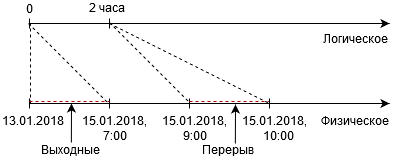
\includegraphics[width=0.7\linewidth]{pics/scheduleAxes.png}
	\caption{Пример отображения оси логического на ось физического времени}
	\label{fig:axes}
\end{figure}

\indent Как было сказано ранее, из-за того что рабочее время является дискретным, мы не имеем возможности просуммировать начальную дату и значение поданного логического времени.
Это ведет к тому, что необходимо синхронизировать логическое и физическое время,и это достигается путем последовательного периодического отображения конкретного логического времени на физическое (см. \ref{fig:axes}).
Это подразумевает под собой наличие двух массивов чисел или ``осей'':

\begin{itemize}
	\item оси логического времени, которая начинается с нуля и единица которой соответствует одной секунде (необходимости в более точном отображении нет);
	\item оси физического времени, на которой может быть отложено любая дата физического времени, отсчет которой начинается 1 января 1970 года 00:00:00 (эпоха Unix).
\end{itemize}

\indent Особенностью оси физического времени является наличие на ней ``выколотых'' промежутков времени, в которые работа не ведется и операции не выполняются, следовательно, об этих промежутках системе необходимо знать, что подразумевает данную информацию как входные данные.
% Они передаются системе в виде структуры данных, которая далее будет называться ``конфигурацией модуля''.\\

\indent Входными данными для модуля являются:

\begin{itemize}
	\item дата с которой необходимо начинать отсчет;
	\item логическое время, которого необходимо достигнуть;
	\item конфигурация модуля.
\end{itemize}

\indent Дата является точкой на физической оси, на которую будет отображаться нуль логической. Представляет собой количество секунд, прошедшее с начала эпохи Unix.

\indent Логическое время~-~количество секунд, которое должно быть отложено на логической оси. В силу непрерывности физической оси, каждой логической точке сопоставляется отрезок на физической оси, сопоставляется пара чисел - границ данного отрезка.

\indent Конфигурация модуля~-~вспомогательные данные используемые для определения модулем какие промежутки необходимо пропускать в процессе работы.
Состоит из данных о рабочем графике занятого персонала (интервалы рабочего времени), шаблонном расписании на неделю (например, суббота, воскресенье - выходные, пятница - ``короткий'' день, остальные - стандартные рабочие дни) и набор информации о датах, которые являются днями-исключениями и соответствующей информацией о графике работы в данные дни.
% \subsection{Результат работы}

% \subsection{Реализация}
\indent После запуска, модуль получает параметры и совершает проверку последних на корректность и непротиворечивость (например, если два дня имеют пересечения временных промежутков то они противоречивы, ведь ресурс не может работать одновременно в двух сменах) как в рамках смен одного так соседних дней.
Далее производится определение режима работы: прямой, обратный расчет или проверка времени:

\begin{itemize}
	\item прямой расчет - задается дата начала отсчета, логическое время и расчет ведется до нахождения даты окончания работ (см \ref{fig:straightCalc});
	\item обратный расчет - задается дата дедлайна, логическое время и расчет ведется до нахождения времени начала работ(см \ref{fig:reverceCalc});
	\item проверка времени - задается дата и логическое время равное нулю, что запускает оба предыдущих расчета пока не будет найдено первое ненулевое время в обоих направлениях от даты начала расчета(см \ref{fig:checkCalc}).
\end{itemize}

\begin{figure}[ht!]
	\centering
	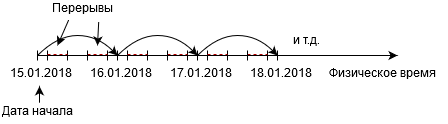
\includegraphics[width=0.7\linewidth]{pics/scheduleStraightCalc.png}
	\caption{Схема прямого расчета}
	\label{fig:straightCalc}
\end{figure}

\begin{figure}[ht!]
	\centering
	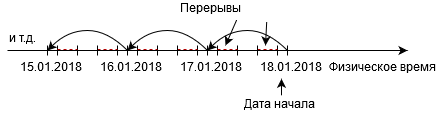
\includegraphics[width=0.7\linewidth]{pics/scheduleReverceCalc.png}
	\caption{Схема обратного расчета}
	\label{fig:reverceCalc}
\end{figure}

\begin{figure}[ht!]
	\centering
	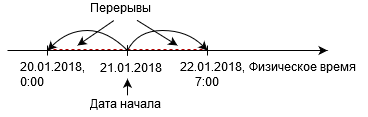
\includegraphics[width=0.7\linewidth]{pics/scheduleCheckCalc.png}
	\caption{Схема проверки времени}
	\label{fig:checkCalc}
\end{figure}

\indent Выбрав режим работы сбрасывается счетчик текущего логического времени до нуля и счетчик текущего физического времени до стартовой даты. Затем итеративно, пока текущее логическое время не превысит необходимое производится поиск следующей даты.
Алгоритмически, поиск даты работает следующим образом:

\begin{enumerate}
	\item[\mylabel{itm:point1}{1})] определяются интервалы рабочих смен относящихся к текущему дню:
	      \begin{enumerate}
		      \item[а)] при отсутствии таковых, к текущей дате прибавляется один день и затем возврат к п.\ref{itm:point1}.
	      \end{enumerate}
	\item[2)] отсортированные в порядке возрастания интервалы последовательно перебираются и их длительности прибавляются к текущему логическому и физическому времёнам:
	      \begin{enumerate}
		      \item[а)] при превышении текущим логическим временем необходимого, переход к п.\ref{itm:point3};
		      \item[б)] если все интервалы были просуммированы, но необходимое логическое время не превышено - переход к п.\ref{itm:point1};
	      \end{enumerate}
	\item[\mylabel{itm:point3}{3})] разность текущего и необходимого логического времён вычитается из физического времени, при этом сохраняя данное значение как левую (правую при обратном расчете) границу и продолжается расчет для выявления правой (левой) границы промежутка.
\end{enumerate}

\begin{figure}[ht]
	\centering
	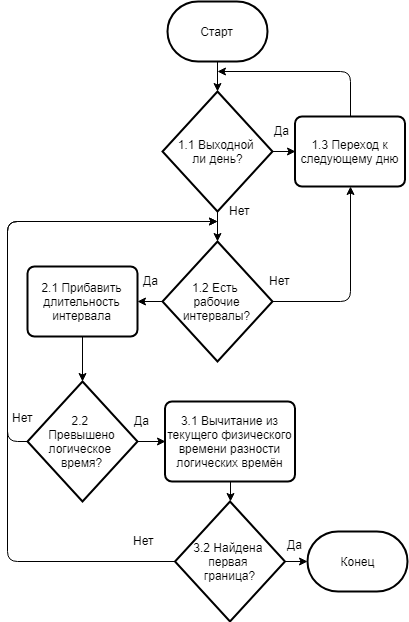
\includegraphics[width=\linewidth]{pics/scheduleSchema.png}
	\caption{Блок-схема модуля}
	\label{fig:schema}
\end{figure}

\indent Определение интервалов рабочего времени происходит взятием даты из текущего физического времени, после чего начинается определение принадлежности данной даты к перенесенным датам после чего есть два варианта развития ситуации:

\begin{itemize}
	\item дата является перенесенным днем и модуль получает информацию о расписании которое нужно применить;
	\item дата не является перенесенным днем и получение информации происходит исходя из того, каким днем недели является данная дата.
\end{itemize}

\begin{figure}[ht]
	\centering
	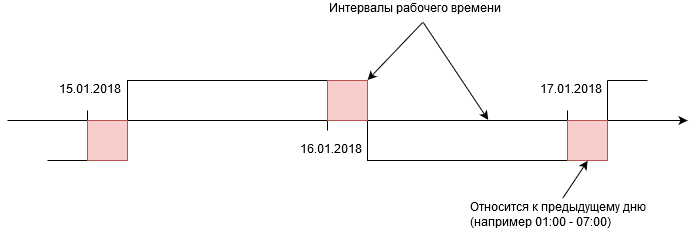
\includegraphics[width=\linewidth]{pics/scheduleIntervals.png}
	\caption{Смещение интервалов рабочего времени относительно рабочего дня}
	\label{fig:intervals}
\end{figure}

\begin{figure}[ht]
	\centering
	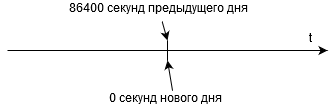
\includegraphics[width=0.6\linewidth]{pics/scheduleTime.png}
	\caption{Граница двух дней}
	\label{fig:time}
\end{figure}

\indent Так как на реальных производственных площадках нередко случается так, что рабочие интервалы, принадлежащие к рабочему дню и сам рабочий день смещены относительно друг друга (см. \ref{fig:intervals}).
При этом возникают трудности с определением интервалов рабочего времени в связи с тем, что для определения используется количество секунд с начала эпохи Unix и до нуля часов нуля минут и нуля секунд нужной даты, по которому, используя инструментарий языка, каким днем недели является нужная дата и, соответственно, задать для нее шаблон рабочего времени.
И если эти трудности практически не влияют на прямой расчет, то с обратным все немного сложнее.
Так как одном дне 86400 секунд и, если рассматривать границу двух дней (см. \ref{fig:time}), то 86400 секунда предыдущего дня будет равна или тем же что и нулевая секунда нового дня.
Можно сказать, что 86400 - левый предел, а 0 - правый предел в данной точке (особенно если изображать в виде окружности).
Но, в связи с тем, что данная недетерминированность присутствует лишь при рассмотрении человеком данной ситуации, а система может распознавать диапазон от 0 до 86399 секунд, то для определения интервалов рабочего графика (при обратном расчете) используется именно величина в 86399 секунд, при условии, что данное допущение не влияет на расчет, как последняя секунда текущего дня.

\begin{figure}[ht]
	\centering
	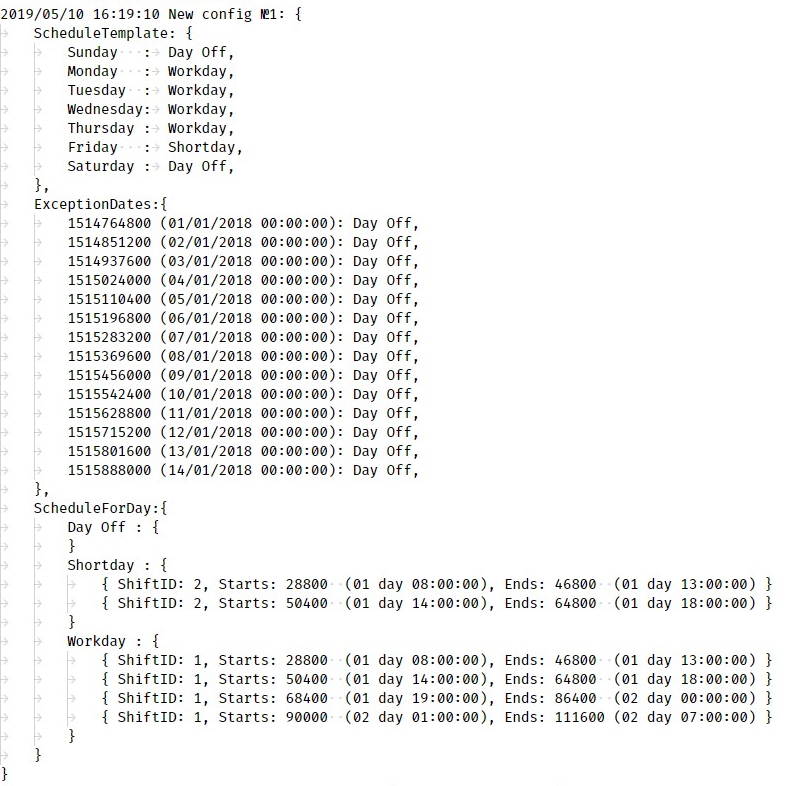
\includegraphics[scale=0.6]{pics/scheduleConfigExample.png}
	\caption{Пример конфигурации модуля}
	\label{fig:config}
\end{figure}

\indent Возвращаясь к пункту \ref{itm:point3} алгоритма, при нахождении нужного времени, работа модуля не прекращается, а ведется до момента нахождения второй границы промежутка, на который отображается необходимое логической время.

\indent Как было сказано ранее - физическое время непрерывно, а следовательно когда производится отображение на него логического времени, в результате должен получиться промежуток (см. \ref{fig:axes}), который и характеризуют две границы.
Эта пара чисел, характеризующие начало и конец отрезка которые отображаются на логическую ось в точке, значение которой равно входному логическому времени и являются выходными данными данного модуля.

\begin{figure}[ht]
	\centering
	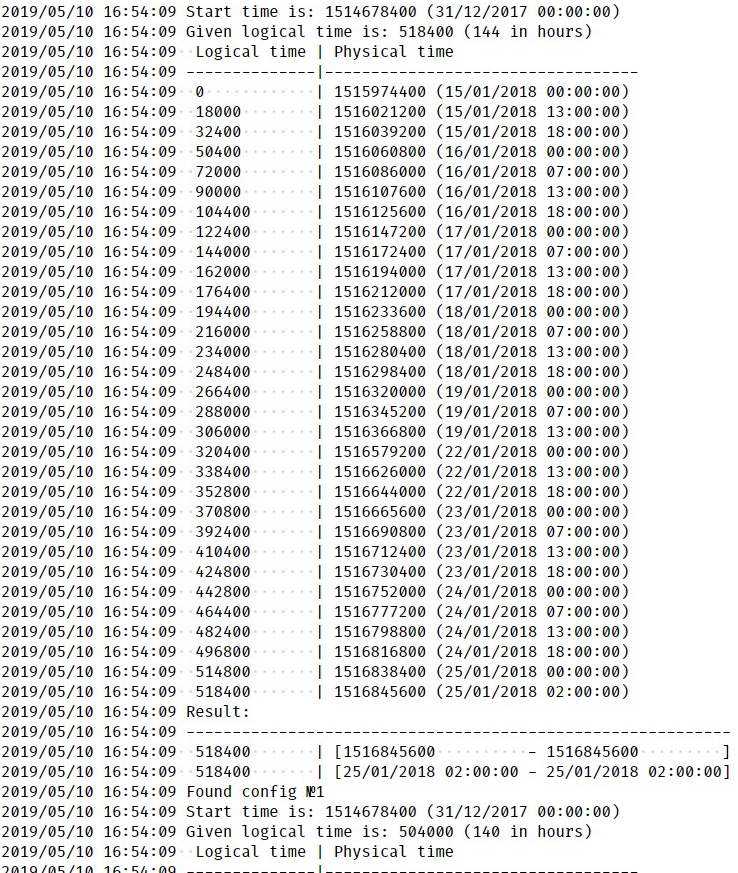
\includegraphics[scale=0.6]{pics/scheduleEvalExample.png}
	\caption{Пример прямого расчета модулем}
	\label{fig:eval1}
\end{figure}

\indent В результате работы над модулем были написаны тесты и проведено тестирование, результаты одного из которых можно увидеть на изображениях \ref{fig:config} и \ref{fig:eval1}.
На \ref{fig:config} изображена конфигурация модуля, которая показывает как производится совмещение логического и физического дня, обработка перенесенных дней.
На \ref{fig:eval1}, перед расчетом нового отображения, можно отметить, что при использовании той же конфигурации не производится ее повторный вывод в лог, что позволяет сократить его длину, а следовательно улучшить читаемость.
Рисунок \ref{fig:eval1} показывает итеративный процесс как результат прибавления каждого нового интервала к текущему времени.

\begin{figure}[ht]
	\centering
	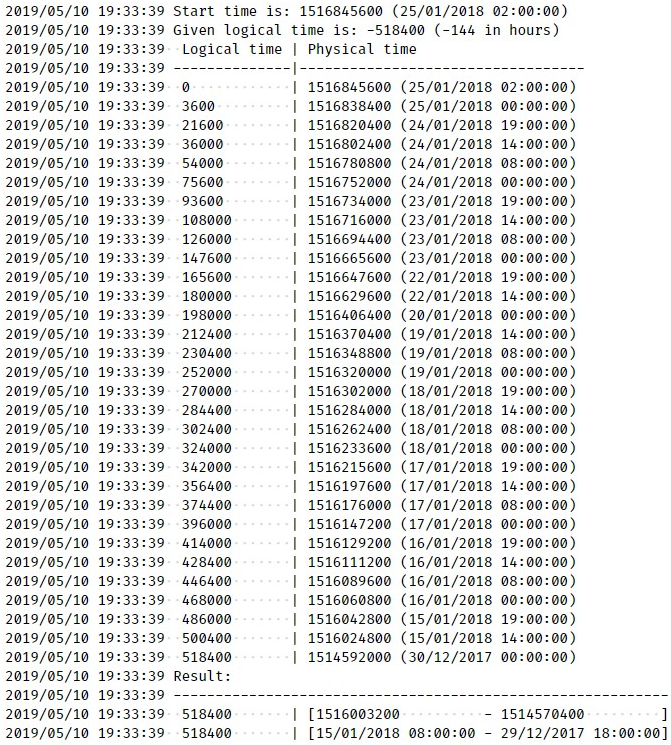
\includegraphics[scale=0.6]{pics/scheduleRevertEvalExample.png}
	\caption{Пример обратного расчета модулем}
	\label{fig:revEval}
\end{figure}

\indent Также были проведены тесты обратного расчета и проверки времени, результаты которых можно видеть на изображениях \ref{fig:revEval} и \ref{fig:checkEval}.
Пояснение к проверке даты: тут используется конфигурация, когда 2 января является выходным, проверка которой и производится, что позволяет продемонстрировать работу данного решения.

\begin{figure}[hb]
	\centering
	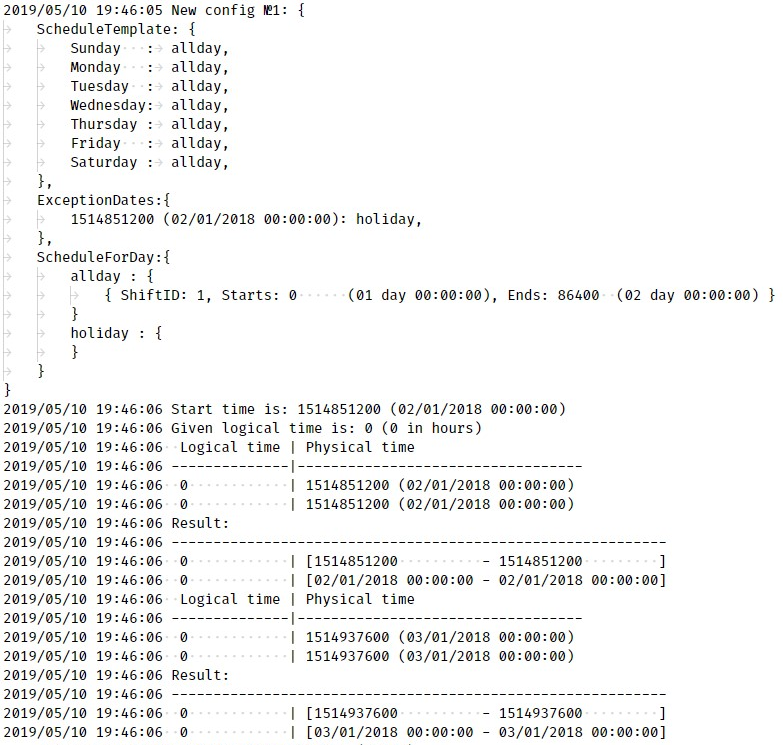
\includegraphics[scale=0.6]{pics/scheduleCheckDateEval.png}
	\caption{Пример проверки модулем времени}
	\label{fig:checkEval}
\end{figure}


% Так как расчет расписания — это итеративный процесс, то в рамках разработки было выделено понятие временной линии (прямой) – это «линия» на которой для каждой точки, которая является абстрактной величиной времени выполнения операции, сопоставляются две даты соответствующие данной абстрактной величине времени с учетом расписания. Первая дата является концом данной операции, вторая – началом следующей. Данное разделение было использовано, потому как все время что между ними также относится к данной точке, а значит каждой точке, из-за непрерывности времени, соответствует бесчисленное множество точек на временной прямой, что может быть лишь ограничено двумя границами – временем начала и конца данного отрезка.
